\chapter{Vorgehensweise und Implementierung}

\section{Themenfindung}
Die zunehmende Digitalisierung und der technologische Fortschritt eröffnen vielfältige Einsatzmöglichkeiten für Methoden der künstlichen Intelligenz (KI). Besonders im Bildungsbereich entsteht dadurch die Chance, Prozesse zu optimieren und Lehrkräfte bei Routineaufgaben zu entlasten.

Vor diesem Hintergrund wurde das Thema dieser Arbeit gewählt. Ziel ist es, das Potenzial von KI-gestützten Verfahren im Kontext der automatisierten Auswertung studentischer Programmierlösungen zu untersuchen. Durch die Clusterung ähnlicher Lösungen können neue Ansätze für Feedbackprozesse entwickelt werden, die eine effizientere und gezieltere Betreuung von Studierenden ermöglichen.


\section{Recherche und Vorbereitung}
Zu Beginn wurden diverse Quellen herausgesucht, die sich im Rahmen dieses Themas bewegen. Besonders oft stach dabei der k-Means Algorithmus heraus oder wie dieser als Grundlage für erweiternde Algorithmen wie den InvAASTCluster (vgl. \cite{Orvalho.28.06.2022}) oder AsanasCluster (vgl. \cite{Paiva.2024}) benutzt wurde, um bessere Ergebnisse zu liefern. Anhand eines Rankings wurde die Relevanz der Quellen festgelegt, um das weitere Vorgehen einzugrenzen.

Andere Methoden wie der Caliński-Harabasz Index oder der Silhouette Score wurden erwähnt, die zur Evaluation des Clusterings dienen. Es wurde klar, dass der Verlauf von studentischen Programmierlösungen bis zu nutzbaren Daten zur Feedbackgenerierung ein mehrschrittiger Prozess ist.

Der folgende Abschnitt, beschreibt die Entstehung des Programms bzw. einer Pipeline, die die benötigten Prozessschritte beeinhaltet, um dies zu erreichen.


\section{Implementierungsverlauf}
\subsection{Erster Implementierungsabschnitt}
Um einen mehrschrittigen Prozess zu vereinen, eignete sich das Prinzip einer Pipeline, in der nacheinander Algorithmen ablaufen, dessen Eingabewerte vom vorherigen Algorithmus abhängen und dessen Ausgabewerte dem Nächsten folglich wieder als Eingabe dienen.


\subsubsection*{Dateien laden}
Als erstes musste es eine Möglichkeit geben die Java-Dateien der studentischen Programmierlösungen einlesen zu können. Diese wurden als Datensätze durch den betreuenden Prof. Dr. Striewe bereitgestellt.

Der Datensatz an denen das Programm fortlaufend getestet wurde, bestand aus mehreren Überordnern und final aus drei Java-Dateien und einer Text-Datei, welche den Studierenden vorgegeben waren und vervollständigt werden mussten. Jedoch soll die Menge der Java-Dateien keine überwiegende Rolle spielen.

Das Programm musste also in der Lage sein Ordner zu durchsuchen und Java-Dateien zu erkennen. Dies ermöglichte eine Methode des ersten implementierten Moduls \texttt{data\_loader.py}. Es extrahierte Quellcode-Text und speicherte pro Datei Code-Schnipsel (Code Snippets) in eine Liste und gab diese an die Pipeline zurück.

Anfangs entstanden durch problematische Zeichen innerhald der Java-Dateien Fehlermeldungen, welche jedoch einfachheitshalber ignoriert werden.


\subsubsection*{Vektorrepräsentation}
Als nächstes folgte ein Modul zum einbetten dieser Code Snippets bzw. zum dessen repräsentieren durch hochdimensionale Vektoren. Dies war notwendig um sie für Clustering-Algorithmen vorzubereiten. 

Dafür wurde das Modul \texttt{embedding\_model.py} erstellt, welches vortrainierte Sprachmodelle aus der Transformers-Bibliothek\footnote{\url{https://huggingface.co/docs/transformers}} von Python (hier CodeBERT) und passende Tokenizer, die den Code vorbereitend für den Transformer in Tokens zerlegt, importiert.

Anhand einer Methode werden die Code Snippets in numerische Vektoren umwandelt (Embeddings). Alle enstandenen Embeddings wurde anschließend jeweils an die Pipeline zurückgegeben und in eine Liste abgespeichert.


\subsubsection*{Clustering}
Nun mussten die Embeddings geclustert werden. Das entsprechend erstellte Modul \texttt{clustering\_engine.py} importierte dafür die beiden Cluster Algorithmen k-Means aus der scikit-learn Bibliothek\footnote{\url{https://scikit-learn.org/stable/modules/generated/sklearn.cluster.KMeans.html}} für maschinelles Lernen und HDBSCAN aus der separaten HDBSCAN Python-Bibliothek\footnote{\url{https://hdbscan.readthedocs.io/en/latest/api.html\#hdbscan.hdbscan.HDBSCAN}}. An die Pipeline werden schließlich mit Markierungen (Labels) versehene Cluster zurückgegeben.


\subsubsection*{Evaluationsmetriken}
Anschließend wurde ein Evaluationsverfahren eingebaut, um die Qualität der Cluster zu bewerten. Dafür wurde das Modul \texttt{evaluation\_metrics.py} implementiert. Darin wird jeder Cluster nach den Evaluationsmetriken Silhouette Score\footnote{\url{https://scikit-learn.org/stable/modules/generated/sklearn.metrics.silhouette_score.html}}, Caliński-Harabasz Index\footnote{\url{https://scikit-learn.org/stable/modules/generated/sklearn.metrics.calinski_harabasz_score.html}} und den Davies-Bouldin Index\footnote{\url{https://scikit-learn.org/stable/modules/generated/sklearn.metrics.davies_bouldin_score.html}} getestet, welche ebenfalls aus der scikit-learn Bibliothek importiert wurden. Zurückgegeben wird ein Dictionary mit den drei Zahlenwerten der Evaluationsmetriken.


\subsubsection*{Tests, Optimierungen und Dokumentation}
Jedes implementierte Modul wurde einzeln getestet. Dazu wurden das Ergebnis und die Zeit, welche für den jeweiligen Prozessschritt notwendig waren durch print-Anweisungen ausgegeben. Dabei stellte sich heraus, dass Embedding und besonders Imports relativ viel Zeit in Anspruch nahmen.

Da die zu testenden Datensätze teilweise aus mehreren hunderten Dateien bestanden, wurde dazu caching der Embeddings eingeführt, um das Testen des Zusammenspiels der einzelnen Module zu beschleunigen. Versuche die Imports durch lazy loading zu beschleunigen waren in diesem Fall nur geringfügig merkbar.

Des Weiteren wurde eine Requirements.txt-Datei erstellt. Diese beeinhaltet sämltiche Information über die aktuell im Projekt benutzen Versionen der importierten Bibliotheken. Sie sorgt, dass für andere Nutzende gleiche Bedingungen wie auch in der Entwicklung herrschen, um ein lauffähiges Programm zu gewährleisten.

Die noch später hinzugefügte Datei HowToInstall.txt dient zusätzlich als Schritt-für-Schritt-Anleitung. Weiterhin wurde eine config.yaml-Datei hinzugefügt. Diese diente als zentrale Ansprechquelle der Pipeline für Parameter.


\subsubsection*{Dimensionsreduktion}
Zu diesem Zeitpunkt war ein Visualisierungs-Modul geplant, um die Clusterungen sichtbar zu machen, doch bevor es sinnvoll eingesetzt werden konnte, wurde noch ein weiterer Prozessschritt eingebunden, das Dimensionsreduktionsverfahren bzw. dessen Algorithmen. Das entsprechende Modul \texttt{dimensionality\_reducer.py} importiert auch hier Algorithmen aus der scikit-learn Bibliothek, die Principal Component Analysis (PCA)\footnote{\url{https://scikit-learn.org/stable/modules/generated/sklearn.decomposition.PCA.html}} und t-Distributed Stochastic Neighbor Embedding (t-SNE)\footnote{\url{https://scikit-learn.org/stable/modules/generated/sklearn.manifold.TSNE.html}}. Der dritte Algorithmus Uniform Manifold Approximation and Projection (UMAP)\footnote{\url{https://umap-learn.readthedocs.io/en/latest/}} stammt aus der eigenständigen UMAP-learn Bibliothek. 

Dieser Prozessschritt findet zwischen Embedding und Clustering statt. Er reduziert die Embeddings bzw. die hochdimensionalen Vektoren in ihren Dimensionen (hier zu 2D oder 3D), welche danach zur Clusterung weitergereicht und dadurch auch besser als menschlicher Betrachter in einem Diagramm beobachtet werden können.


\subsubsection*{Visualisierung}
Schließlich wurde noch das Modul \texttt{cluster\_plotter.py} implementiert, welches anhand der dimensionsreduzierten Embeddings und der aus dem Clustering hervorgegangenen Labels ein statisches Diagramm (engl. plot) in einem separatem Fenster erstellt (Beispiel-Clusterung in Abbildung \ref{abb:E-CD}). Hierfür wurden aus der Matplotlibs Bibliothek die Plotting-Module pyplot\footnote{\url{https://matplotlib.org/stable/api/pyplot_summary.html}} und \texttt{mpl\_toolkits.mplot3d}\footnote{\url{https://matplotlib.org/stable/gallery/mplot3d/2dcollections3d.html\#sphx-glr-gallery-mplot3d-2dcollections3d-py}} importiert, die für 2D- und 3D-Visualisierung (falls gewünscht) zuständig sind.

Die zuvor erstellten Module gleichten sich durch ihre einheitlichen Klassenstruktur, da jedoch für dieses Modul keine Zwischenspeicherung von Zuständen anhand einer Instanz notwendig war, wurden dessen Methoden statisch definiert.


\subsubsection*{Pipeline}
Die Pipeline besteht zu diesem Zeitpunkt aus folgendem Ablauf:

\textbf{Daten laden} $\rightarrow$ \textbf{Einbetten} $\rightarrow$ \textbf{Dimensionen reduzieren} $\rightarrow$ \textbf{Clustern} $\rightarrow$ \textbf{Evaluieren} $\rightarrow$ \textbf{Visualisieren}

\begin{figure} %[hbtp]
	\centering
	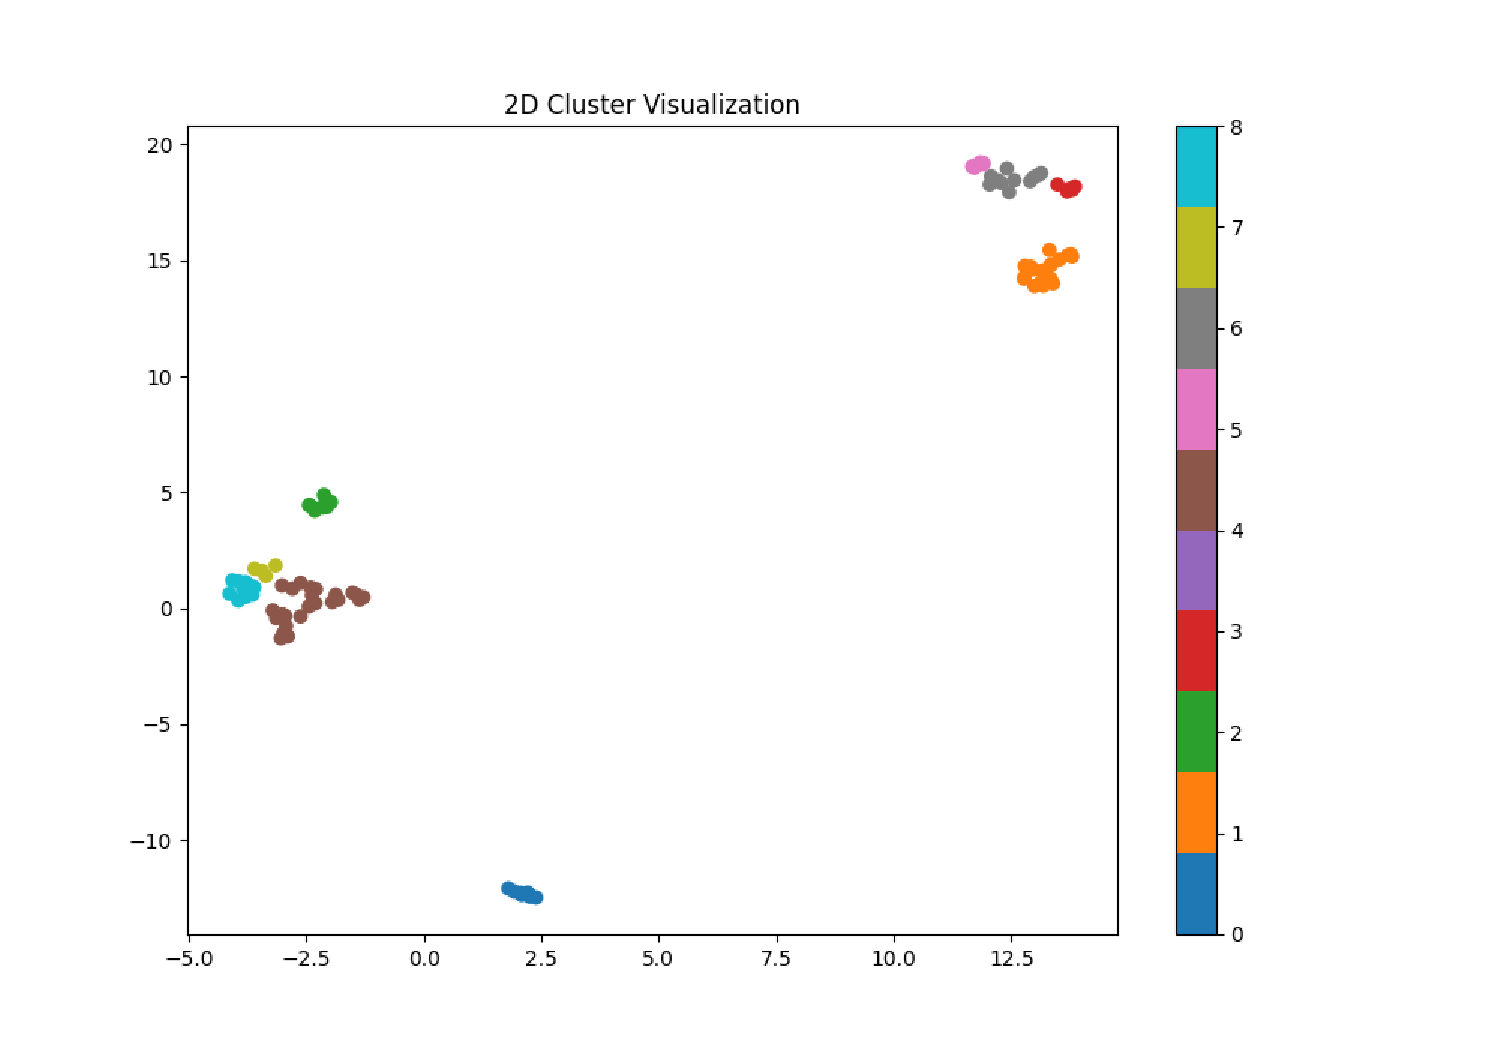
\includegraphics[width=0.8\textwidth]{images/Erstes Clustering-Diagramm.pdf}
	\caption{Zweidimensionales Clustering-Diagramm einer Clusterung von 147 Java-Dateien. Die unterschiedlichen Farben kennzeichnen die Zugehörigkeit der Punkte zu einem Cluster. Am rechten Rand sind die benutzten Farben in einer Farbskala angeordnet.}
	\label{abb:E-CD}
\end{figure}


\subsection{Zweiter Implementierungsabschnitt}
\subsubsection*{Interaktive Diagramme}
In Abbildung \ref{abb:I-CD} sind zwar farbige Punkte in unterschiedlicher Anzahl pro Cluster zu erkennen, jedoch wurden keine Labels angezeigt, die Informationen über die Punkte anzeigen sollten. Als vorbereitender Schritt für weiterführende Prozesse zur automatischen Feedbackgenerierung, müssen sie zumindest zum Testen visuell zuordenbar sein.

Aus diesem Grund wurde ein weiteres Modul zur Visualisierung implementiert. Das entstandene Modul \texttt{interactive\_plot.py} nahm dafür wieder Embeddings, Labels und zustätzlich noch den Namen der aktuellen Java-Datei entgegen, die im \texttt{data\_loader.py}-Modul gespeichert wurde.

Dazu wurden aus der Python-Bibliothek die Module Pandas\footnote{\url{https://pandas.pydata.org/docs/}} und Plotly Express\footnote{\url{https://plotly.com/python/plotly-express/}} importiert, die einerseits zur Erstellung von Tabellenstrukturen (DataFrames) und andererseits für einfache und interaktiave Diagramme zuständig sind. Ausgeführt, öffnete sich ein Fenster im Webbrowser mit einem von der Gestalung her ähnlichem Diagramm wie in der statischen Variante (\ref{abb:E-CD}).

\begin{figure} %[hbtp]
	\centering
	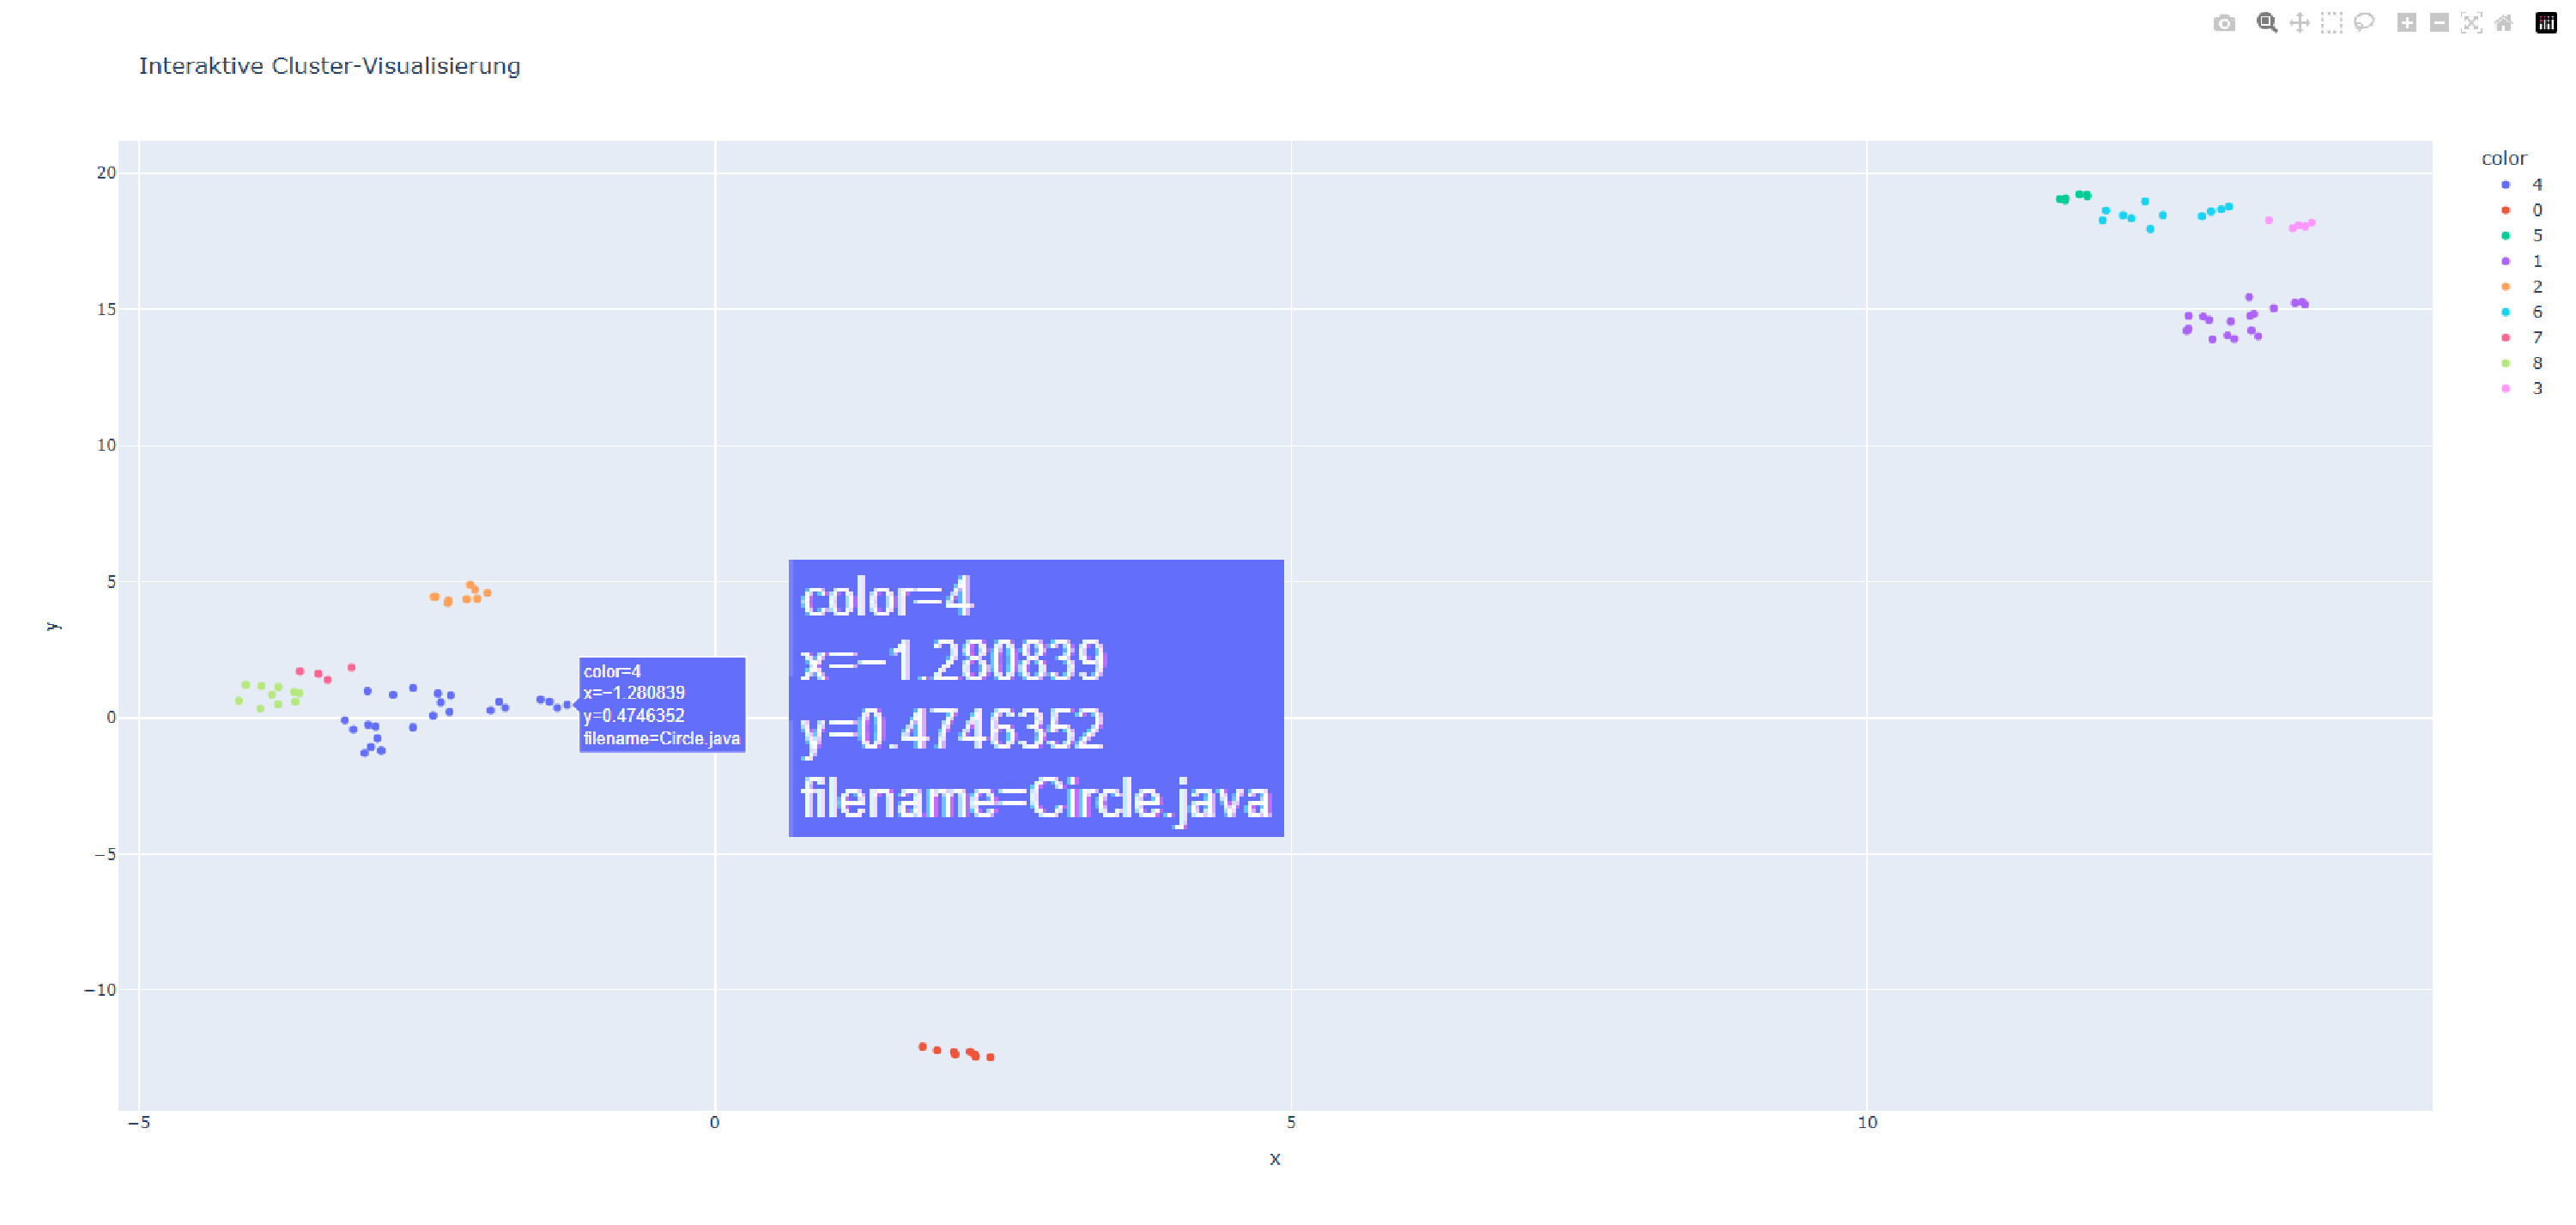
\includegraphics[width=1.0\textwidth]{images/Interaktives Clustering-Diagramm.pdf}
	\caption{Interaktives Clustering-Diagramm einer Clusterung von 147 Java-Dateien. Durch das Halten der Maus über die Punkte werden Informationen über sie angezeigt (im Bild wiederholt vergrößert dargestellt). Am rechten Rand sind die Mengen der Cluster angezeigt.}
	\label{abb:I-CD}
\end{figure}


\subsubsection*{Probleme bei der Cluster-Konsistenz und getroffene Maßnahmen}
Beim mehrmaligen Austesten verschiedener Dateimengen und Überprüfen der ausgegeben Punkte, fiel auf, dass Cluster bei größeren Datenmengen nicht mehr konsistent sind, obwohl akzeptable Ergebnisse im Evaluationsmetriken erreicht wurden. Genauer genommen wurden vereinzelt unterschiedliche Dateien in einem gemeinsamen Cluster platziert (gezeigt in \ref{abs:C-u-D-i-e-D} in Abschnitt Forschungsergebnisse). So kamen beispielsweise Point.java-Dateien in einem Cluster mit sonst nur Circle.java-Dateien vor.

Da Clustering-Algorithmen nach ähnlicher Syntax und Semantik clustern, kann solch ein Verhalten durchaus vor kommen, ist hier jedoch nicht von praktischen Nutzen. Andererseits könnten ebenso Fehler in den Algorithmen oder Inkonsistenzen in den gegebenen Datensätzen die fehlerhafte Clusterung verursachen. Selbst Dateien die abhängig von der gestellten Aufgabe zu den Einreichungen bereits gegeben waren, nicht bearbeitet werden sollten und überall identisch waren, wurden in verschiedenen Clustern angeordnet.

Als erste Maßnahme gegen dieses Problem, wurden die nicht zu bearbeitenden Dateien ignoriert, indem nicht mehr allgemein nach.java-Dateien gesucht wird, sondern nur noch nach bestimmten Namen. 

Im weiterem Verlauf wurde zudem in der Pipeline eine Schleife ergänzt, die die Prozesse ab Embedding bis zur Visualisierung für die gewünschten, in der Konfigurationsdatei festgelegten Namen bzw. Java-Dateien wiederholt. Dadurch werden gemischte Cluster verhindert und für jede unterschiedene Java-Datei ein Diagramm erstellt.

Weiterhin ist beim Testen einer niedriger Anzahl von Dateien (\(n \leq 4\)) aufgefallen, dass der Embedding-Algorithmus nicht mehr funtkioniert, jedoch ist solche eine Clusterung ohnehin nicht von Nutzen.


\subsubsection*{Experimentierungspipeline}
Um die Evaluationsmetriken einfach testen zu können, wurde eine separate Experimentierungspipeline erstellt. Der Vorteil bestand darin, dass die verschiedenen Kombinationen der Dimensionsreduktions- und Clustering-Algorithmen mit ihren Parametern über Dictionaries innerhalb der Pipeline definiert wurden. Die Evaluationsergebnisse wurden anschließend in einer CSV-Datei im Projektverzeichnis festgehalten.

In den Tabellen \ref{tab:EI-EV-20} und \ref{tab:EI-EV-160} im Abschnitt Forschungsergebnisse wurde gezeigt, welche Algorithmen-Kombination für verschiedene Dateimengen geeignet sind.


\subsubsection*{Visuelle Erweiterung}
Um den Punkten im Diagramm mehr Informationen entnehmen zu können, wurde neben den Dateinamen nun noch der Name des Einreichungsordners hinzugefügt. Da die erreichten Punktzahlen der Einreichungen Teil des Ordnernames sind, konnten die Clusterungen jetzt besser nachvollzogen und überprüft werden. Weiterhin wurde das \texttt{interactive\_plot.py}-Modul um die Option das Diagramm als dreidimensionale Umgebung darzustellen erweitert. Sollten mehrere Cluster im 2D-Diagramm aufeinanderliegen, so kann die dritte Achse bessere Einsicht gewährleisten.


\subsection{Dritter Implementierungsabschnitt}
\subsubsection*{Konkatenation gesuchter Dateien}
Auch wenn für jede durch Namen getrennte Art Datei ein separates Diagramm erstellt wird, besteht die Möglichkeit dass die vollständige Einreichung bzw. Lösung zu den gestellten Aufgaben gesamt betrachtet werden sollte, da es sonst zu verminderter Information führen könnte. Um die Dateien als ein Ganzes zu betrachten, wurde das \texttt{data\_loader.py}-Modul um eine Konkatenations-Funktionalität ergänzt. Die entstandene Methode konkateniert alle gesuchten Java-Dateien eines Einreichungsordners. Der im Diagramm gezeigte Dateiname eines Punktes, setzt sich nun aus den konkatenierten Namen der Dateien zusammen. Die Schleife in der Pipeline die die Prozessschritte für jede gesuchte Art Datei wiederholte, wurde daraufhin entfernt.


\subsubsection*{Probleme bei der Cluster-Visualisierung und Punktzuordnung}
Theoretisch wäre das Programm in der Lage, Embeddings ohne Dimensionsreduktionsalgorithmen zu verarbeiten. Zum Testen wird jedoch weiterhin eine geeignete Visualisierung verwendet, bei der allerdings durch die Anzeige der Ordnernamen pro Punkt ein weiteres Probleme auffiel. So werden konkatenierte Dateien in einen Cluster gesteckt, dessen Ordnernamen sich durch stark variierende Punktzahlen unterscheiden, wie in Abbildung \ref{abb:C-40-K-Pg} zu sehen ist. Auch hier kann solch ein Verahlten durchaus vorkommen, ist aber nicht von praktischen Nutzen, da sich das zu generierende Feedback nach den erreichten Punktzahlen unterscheiden sollte. 

\begin{figure} %[hbtp]
	\centering
	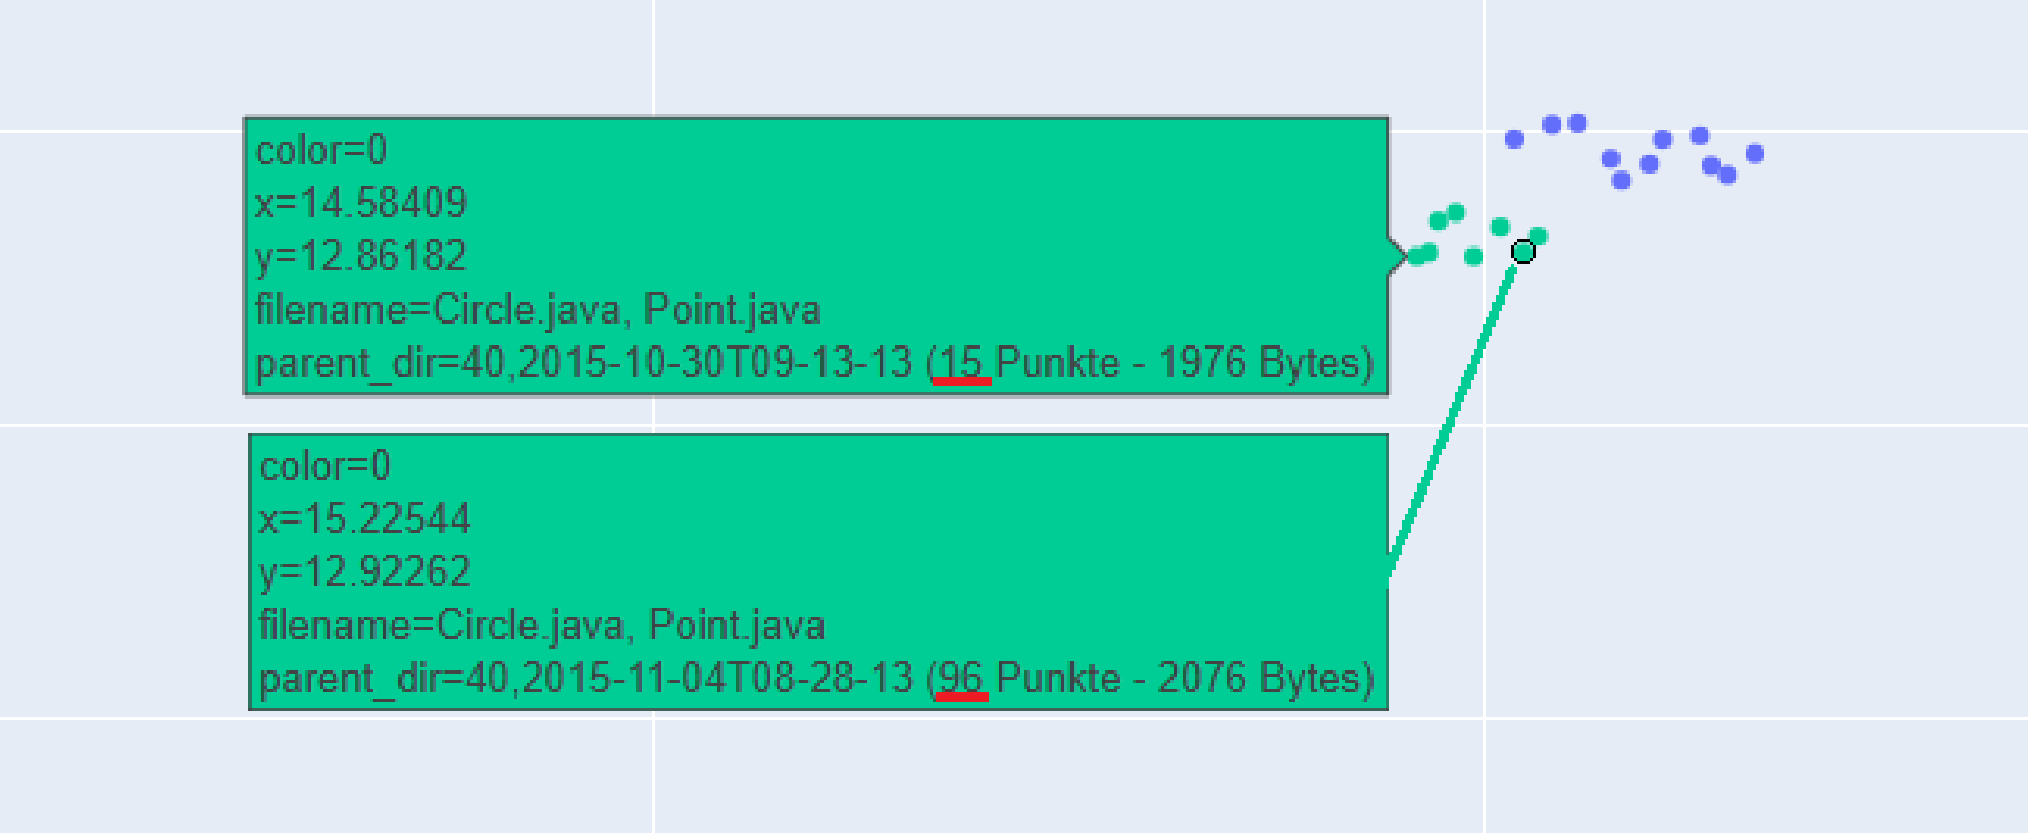
\includegraphics[width=1.0\textwidth]{images/Clusterung - 40 - Konkateniert - Punktzahl gemischt.pdf}
	\caption{Interaktives Clustering-Diagramm einer Clusterung von 80 bzw. 40 konkatenierten Java-Dateien. Die rote Unterstreichung zeigt das Problem gemischert Cluster mit unterschiedlichen Punktzahlen.}
	\label{abb:C-40-K-Pg}
\end{figure}


\subsubsection*{Punktzahlenintervalle}
Um diesem Problem entgegenzuwirken, wurde erneut die Vorgehensweise der wiederholten Prozessschritte mittels einer Schleife angewendet, indem nach Ebenen bzw. Punktzahlenintervallen (Score-Bins) geclustert wird. Es können beliebig viele Intervalle definiert werden (z. B. 0-49, 50-79, 80-89, 90-100), um das Clustering weiter zu präzisieren. Dafür wurde dem \texttt{data\_loader.py}-Modul eine Methode hinzugefügt, die die Punktzahlen aus den Ordnernamen, in denen die Java-Dateien enthalten sind, ausliest.

Weiterhin wurde das Modul \texttt{score\_binning.py} entwickelt, die den ausgelesenen Punktzahlen ein Intervall zuordnet. Anschließend werden in der Pipeline für jedes Intervall bzw. für alle Dateien die zu diesem Bereich gehören, die Prozesschritte ab Embedding wiederholt. Anstatt daraufhin pro Intervall ein Diagramm zu erstellen, wird zur besseren Übersichtlichkeit alle separaten Clusterungen in einem Diagramm visualisiert. Die Ergebnisse der Evaluationsmetriken werden dadurch zwar verfälscht, haben jedoch bereits die geeignetsten Algorithmen-Kombinationen identifiziert und sind daher für den weiteren Verlauf nicht mehr entscheidend.


\subsubsection*{Verarbeitung von Cluster-Ergebnissen}
Um die Dateimenge weiter einzugrenzen, wurde ein zusätzlicher Parameter der Konfigurationsdatei hinzugefügt, der zu exkludierende Dateinamen speichert. Zudem wurden die Cluster-Ergebnisse mittels eines \texttt{report\_generator.py}-Moduls für weiterführende Prozesse vorbereitet, indem sie nach Score-Bins und Cluster sortiert, in eine CSV-Datei abgespeichert werden. Da es pro Studierenden mehrere Einreichungen geben kann, wurde zudem der Überordnername ergänzt. Folgende Auflistung zeigt diese Struktur. Ein Element eines Clusters besteht aus: Überordner - Einreichungsordner - (konkatenierte) Java-Dateien.

\subsection*{Score-Bin: 0-49}
\begin{itemize}
  \item \textbf{Cluster 0:}
  \begin{itemize}
    \item 0D01AAB9 -- 2015-11-03T19-55-35 (28 Punkte -- 1485 Bytes) -- Circle.java, Point.java
    \item 0D1C6395 -- 2015-10-30T09-10-34 (15 Punkte -- 1976 Bytes) -- Circle.java, Point.java
  \end{itemize}
  \item \textbf{Cluster 1:}
  \begin{itemize}
    \item 0B87094E -- 2015-11-03T13-16-47 (0 Punkte -- 1983 Bytes) -- Circle.java, Point.java
    \item \dots
  \end{itemize}
  \dots
\end{itemize}

Im folgendem Abschnitt wird die finale Implementierung bzw. dessen Module vorgestellt.

\section{Finale Implementierung}
In Abbildung \ref{abb:C-160-gC} ist die Ordnerstruktur des Projekts zu sehen. Cache-Dateien, welche automatisch von VSC generiert wurden, wurden nicht mit aufgelistet.
\subsection{Pipeline}
Die Pipeline besteht zu diesem Zeitpunkt aus folgenden Hauptbestandteilen:

\textbf{Daten laden} $\rightarrow$ \textbf{Punktzahlenintervalle} $\rightarrow$ \textbf{Einbetten} $\rightarrow$ \textbf{Dimensionen reduzieren} $\rightarrow$ \textbf{Clustern} $\rightarrow$ \textbf{Evaluieren} $\rightarrow$ \textbf{Visualisieren} $\rightarrow$ \textbf{Bericht erstellen}

\subsubsection*{Ablauf}
Zuerst wird die Konfigurationsdatei eingelesen (Abschnitt \ref{abs:config.yaml}, \# load config).

Danach werden für die Funktionalität des Programms unwichtige Warnungen ignoriert, um die Ausgabe übersichtlich zu halten (\# ignore warnings). Sie beziehen sich auf auf veraltete Parameter, eingeschränkte Parallelverarbeitung durch feste zufällige Status (Random States) und automatische Anpassung von Nachbarparametern bei kleinen Datenmengen.

Als nächstes wird der Eingabepfad bestimmt, indem der Pfad der studentischen Einreichungen mit dem des aktuellen Projekts vereint wird (\# dynamically determine path).

Dieser Pfad wird daraufhin neben anderen Parametern zum laden der studentischen Einreichungen genutzt und als Code-Schnipsel abgespeichert (Abschnitt \ref{abs:data-loader}, \# load data).

Danach werden die Punktzahlenintervall vorbereitet (Abschnitt \ref{abs:score-binning}, \# score bins). Die aus den Einreichungsorder extrahierten Punktzahlen werden einem Punktzahlenintervall eingeordnet und sortiert diese dann alphabetisch.

Nun werden vorbereitend ein Embedding-Objekt und der Name der zwischengespeicherten (cached) Embeddings erstellt (\# Embedding object). Zudem werden Listen angelegt, die Informationen über die Einreichungen aus der darauffolgenden Schleife speichert, um sie später in einem Diagramm darstellen zu können (\# save all information \dots).

Folgend wird über alle Punktzahlenintervalle iteriert (\# filter solutions by \dots). Darin werden die Indizes aller Einreichungen über eine Liste gemerkt, dessen Punktzahl im aktuellen Punktzahlenintervall liegt. Bei einer niedrigen Dateimenge, kann nicht sinnvoll geclustert werden. Darum werden Punktzahlenintervalle ignoriert, zu denen weniger als vier Einreichungen zugeordnet werden konnten. Danach werden für die ausgewählten Indizes die passenden Code-Schnipsel, Datei- und Ordnernamen aus den jeweiligen Listen herausgefiltert und in neue Listen für diese Punktzahlenintervalle gespeichert.

Im nächsten Teil der Schleife werden die Embeddings berechnet (Abschnitt \ref{abs:embedding-model}, \# Embedding in loop). Es wird geprüft ob bereits ein Embedding-Cache vorliegt und ob dessen Größe die Anzahl der aktuell zu prüfenden Dateimenge einrahmt. Wenn ja, werden die Embeddings aus dem Cache geladen, ansonsten werden sie neu berechnet und im Cache abgespeichert.

Danach werden nacheinander die Embeddings in ihren Dimensionen reduziert (Abschnitt \ref{abs:dimension-reducer}, \# Dimension reduction), die reduzierten Embeddings geclustert (Abschnitt \ref{abs:clustering-engine}, \# Clustering of the \dots) und diese dann evaluiert (Abschnitt \ref{abs:evaluation-metrics}, \# Evaluation). Anschließend werden alle Daten in der vor der Schleife definierten Listen angehängt (\# save all information \dots).

Nach der Schleife werden die gesammelten Daten in einem Diagramm visualisiert (Abschnitt \ref{abs:advanced-interactive-plot}, \# Advanced interactive plot). Daneben kann noch auf das statische Diagramm zugegriffen werden (dient als Reserve und wird hier nicht genauer erklärt).

Als letztes wird der im Implementierungsverlauf erwähnte Bericht über das Clustering erstellt (Abschnitt \ref{abs:report-generator}, \# Reporting).


\subsubsection*{\texttt{config.yaml}}
\label{abs:config.yaml}
Hier sind alle Parameter gehalten, die in der Pipeline für die verschiedenen Algorithmen gebraucht werden. Es sind die drei vorgestellten Dimensionsreduktionsalgorithmen, sowie die beiden Clustering-Algorithmen mit vollständigen möglichen Parametern angegeben. Weitere Einstellungen werden durch den Parameter "data" getroffen, in den neben Punktzahlen-Intervalle (Score-Bins), die gesuchten Dateien, zu exkludierende Dateien, etc. angegeben werden können. Um Algorithmen zu wechseln, müssen sie entsprechend ent- und auskommentiert werden.


\subsubsection*{\texttt{data\_loader.py}}
\label{abs:data-loader}
Die Klasse nimmt beim Erstellen den Dateinamen, den Pfad zu den studentischen Einreichungen und die zu exkludierenden Datei- und Ordnernamen entegegen. Zudem werden Listen zum speichern aller Dateinamen und Einreichungsordner gespeichert, um sie später im Diagramm anzeigen zu können. Folgende weitere Methoden sind gegeben:
\begin{itemize}
	\item load\_code\_files(): Lädt alle passenden Dateien aus den Einreichungsordnern, liest deren Inhalt, speichert Datei-, Einreichungsordner- und Überordnernamen und entscheidet, ob die Inhalte der Dateien zusammengeführt werden sollen.
	\item get\_scores(): Liest aus den Ordnernamen die Punktzahl heraus und gibt sie als Liste zurück.
	\item get\_filenames() und get\_parent\_dirs(): Ermöglichen Zugriff auf die zwischengespeicherten Datei-, Einreichungsordner- und Überordnernamen.
\end{itemize}


\subsubsection*{\texttt{score\_binning.py}}
\label{abs:score-binning}
Die Klasse enthält die statische Methode bin\_scores(), die eine Liste von Punktzahlen aus get\_scores() des \texttt{data\_loader.py}-Moduls nimmt und anhand der definierten score\_bins aus der Konfigurationsdatei jeder Punktzahl ein passendes Label (z. B. \glqq 90-94\grqq) oder \glqq Unassigned\grqq zuweist, falls sie in kein Intervall passt.


\subsubsection*{\texttt{embedding\_model.py}}
\label{abs:embedding-model}
Die Klasse nimmt beim Erstellen den Namen des Embedding-Modells entgegen und speichert Tokenizer und Transformermodell (hier CodeBERT). Diese erhalten über die Methode get\_embedding() Code-Schnipsel, zerlegen sie weiter in Einheiten und wandeln sie in einen numerischen Vektor (Embedding) um. Anschließend wird das Embedding in einem Numpy-Array zurückgegeben.


\subsubsection*{\texttt{dimension\_reducer.py}}
\label{abs:dimension-reducer}
Ein Objekt der Klasse nimmt den Namen des Algorithmus und ein Dictionary mit Parametern entgegen, welche den Algorithmus manipulieren. Die Methode reduce() nimmt Embeddings entgegen, wendet dann den gewählten Algorithmus darauf an und gibt dimensionsreduzierte Embeddings zurück.


\subsubsection*{\texttt{clustering\_engine.py}}
\label{abs:clustering-engine}
Hier werden die dimensionsreduzierten Embeddings aus der Klasse des Moduls \texttt{dimension\_reducer.py} geclustert und deren Cluster-Zugehörigkeit als Labels zurückgegeben. Der Aufbau ist zudem weitestgehend gleich (siehe Abschnitt \ref{abs:dimension-reducer}).


\subsubsection*{\texttt{evaluation\_metrics.py}}
\label{abs:evaluation-metrics}
Die Klasse enthält die statische Methode evaluate(), welche die dimensionsreduzierten Embeddings und die Clustering-Labels entgegennimmt. Wenn mehr als ein Label bzw. Cluster vorhanden ist, werden die importieren Evaluationsmetriken darauf angewendet, dessen Ergebnisse in einem Dictionary gespeichert und anschließend zurückgegeben.


\subsubsection*{\texttt{advanced\_iteractive\_plot.py}}
\label{abs:advanced-interactive-plot}
Die Klasse enthält eine statische Methode plot(), die die dimensionsreduzierten Embeddings, Clustering-Labels, Datei- und Ordnernamen und Punktzahlenintervalle entgegennimmt. Danach werden diese Daten in eine Tabellenstruktur (DataFrame) umgewandelt und damit dann ein Streudiagramm erstellt. Durch entsprechendes ent- und auskommentieren, kann zwischen zwei- und dreidimensionalen Diagrammen gewechselt werden.


\subsubsection*{\texttt{report\_generator.py}}
\label{abs:report-generator}
Die Klasse enthält eine statische Methode generate\_report(), welche die Datei- und Ordnernamen, Clustering-Labels, Punktzahlenintervalle und den Ausgabepfad entgegennimmt. Über eine Schleife wird für jedes Punktzahlenintervall ein neues Dictionary und darin für jeden Cluster eine Liste erstellt. Danach werden diese Container erneut durchgegangen, um damit eine CSV-Datei nacheinander zu füllen. Anschließend wird die Datei im Ausgabepfad abgespeichert.